\section{手法}

本研究では,クラスタ数推定にX-meansを用いる.そして,X-meansで用いる情報量基準を変更することで,どの情報量基準がクラスタ数推定に有効か検証する.

\subsection{X-means}
X-means$^{5)}$は,データ分布が混合等方Gauss分布から生成されたと想定してクラスタ数推定及び
クラスタリングを行う手法である.
$k$-meansの逐次繰り返しと,BICによる分割停止規準を用いることで,クラスタ数を推定しクラスタリングを実行する.

具体的には以下の手順で行われる.
\begin{enumerate}
    \item クラスタ数$k$を初期化する (通常は$k=2$) .
    \item $k$-meansを実行する.
    \item 次の処理を$j=1$から$j=k$まで繰り返す.
    \begin{enumerate}
        \item クラスタ$j$のBIC$_j$を計算する.
        \item クラスタ$j$に所属するデータに対し,クラスタ数2として$k$-meansを行う.
        \item クラスタ数2としてクラスタリングした結果に対しBIC'$_j$を計算する.
        \item BIC$_j$とBIC'$_j$を比較し,BIC'$_j$が大きければクラスタ数$k$に1を足す.
    \end{enumerate}
    \item 前の処理で$k$が増加した場合は処理2へ戻る.そうでない場合は終了する.
\end{enumerate}

\figurenum{fig:x-means}にX-meansの具体的な動作例を示す.
\figurenum{fig:x-means}aは5つの等方Gauss分布から生成されたデータである.
クラスタ数の初期値$k=2$で$k$-meansを実行後,親と子のBICを計算した結果が\figurenum{fig:x-means}bである.
$k=2$で$k$-meansによりクラスタリングした結果,上の4つのデータの塊と右下の1つの塊にクラスタリングされた.
図中の丸印が親クラスタのセントロイド,ばつ印が子クラスタのセントロイドを表す.
子クラスとは,クラスタ$j$に対しクラスタ数2でクラスタリングした結果得られたクラスタのことである.
また,BIC ($k=1$) が親クラスタのBIC,BIC ($k=2$) が子クラスタのBICを表す.
\figurenum{fig:x-means}bの場合,赤色のクラスタでは子のBICが親クラスタのものに比べ大きく,
紫色のクラスタでは子のBICが親クラスタのものに比べ小さい.
よって親クラスタと子クラスタのBICの大小関係から,赤色のクラスタのセントロイドは2つに分割し,
紫色のクラスタのセントロイドは分割しない.
その結果,クラスタ数が1つ増え,クラスタ数は3となる.
次に,全データに対し,クラスタ数3で$k$-meansを実行し,BICを計算した結果が\figurenum{fig:x-means}cである.
その結果,親クラスタと子クラスタのBICの大小関係からクラスタを1つ増やす.
同様に,\figurenum{fig:x-means}dでは,クラスタ数4で$k$-meansを実行しBIC大小結果を比較し,
クラスタを1つ増やしている.
そして,クラスタ数が収束するまで行った結果が\figurenum{fig:x-means}eである.
この場合,全てのクラスタにおいて親のBICが大きくなっているので,クラスタ数5と推定された.
この推定結果は実際のクラスタ数と一致しており,正確に推定できていることがわかる.

\begin{figure}[htbp]
  \begin{minipage}{0.5\hsize}
    \begin{center}
      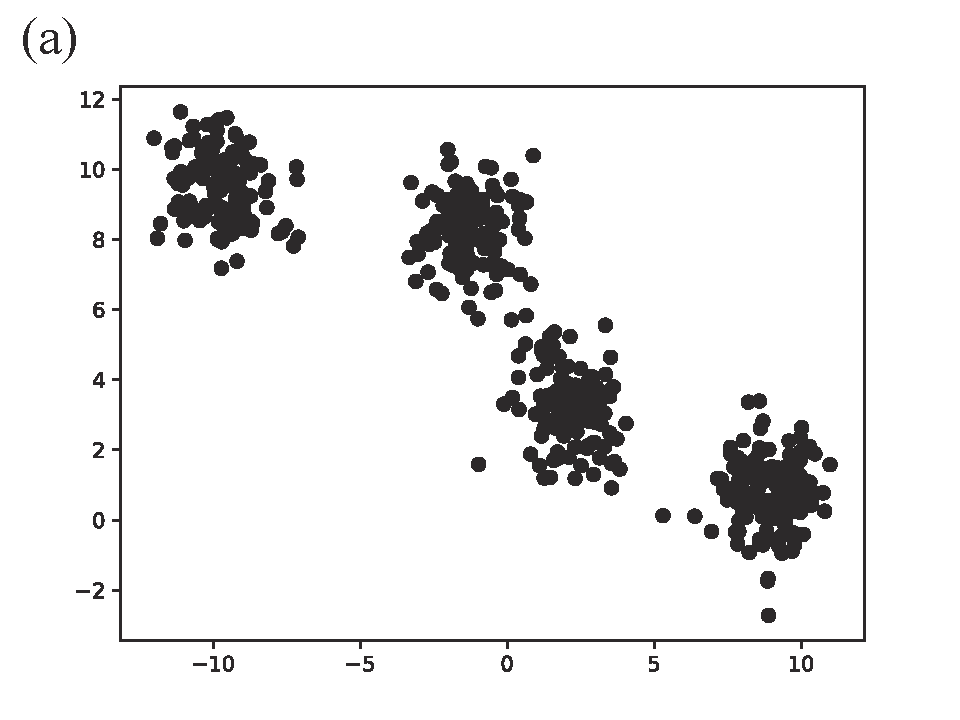
\includegraphics[width=1\linewidth]{img/xmeans/a.pdf}
    \end{center}
  \end{minipage}
  \begin{minipage}{0.5\hsize}
    \begin{center}
      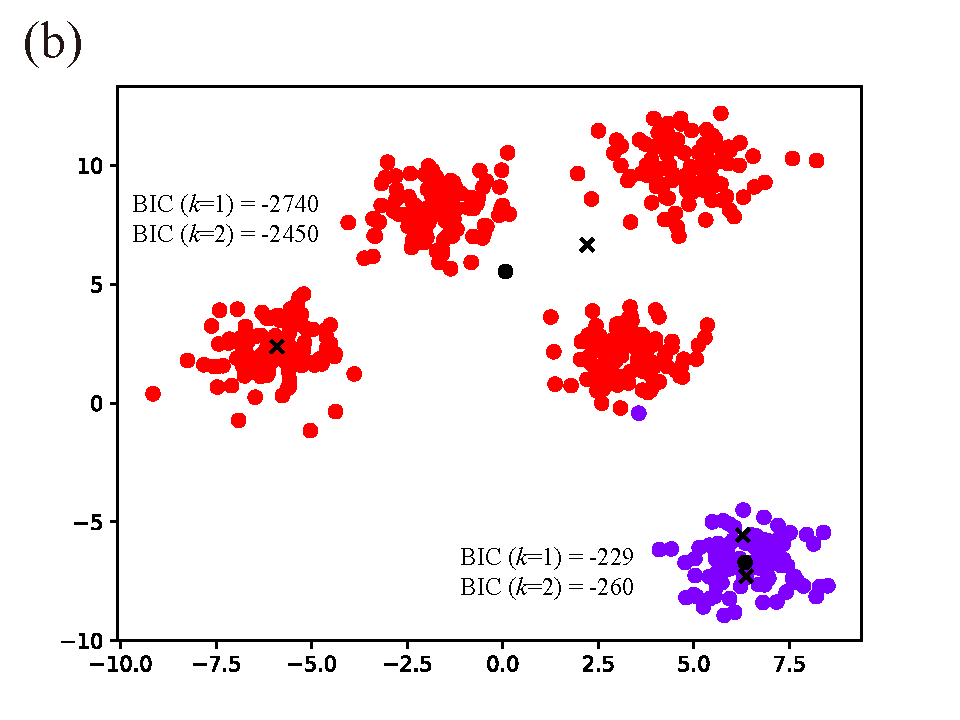
\includegraphics[width=1\linewidth]{img/xmeans/b.pdf}
    \end{center}
  \end{minipage}\\
  \begin{minipage}{0.5\hsize}
    \begin{center}
      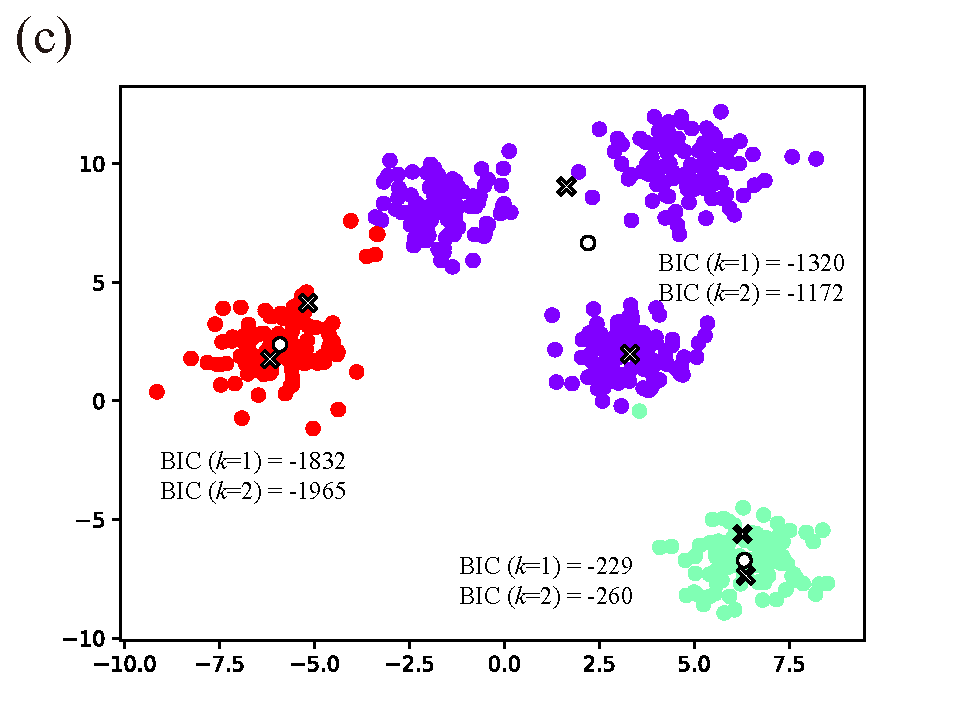
\includegraphics[width=1\linewidth]{img/xmeans/c.pdf}
    \end{center}
  \end{minipage}
  \begin{minipage}{0.5\hsize}
    \begin{center}
      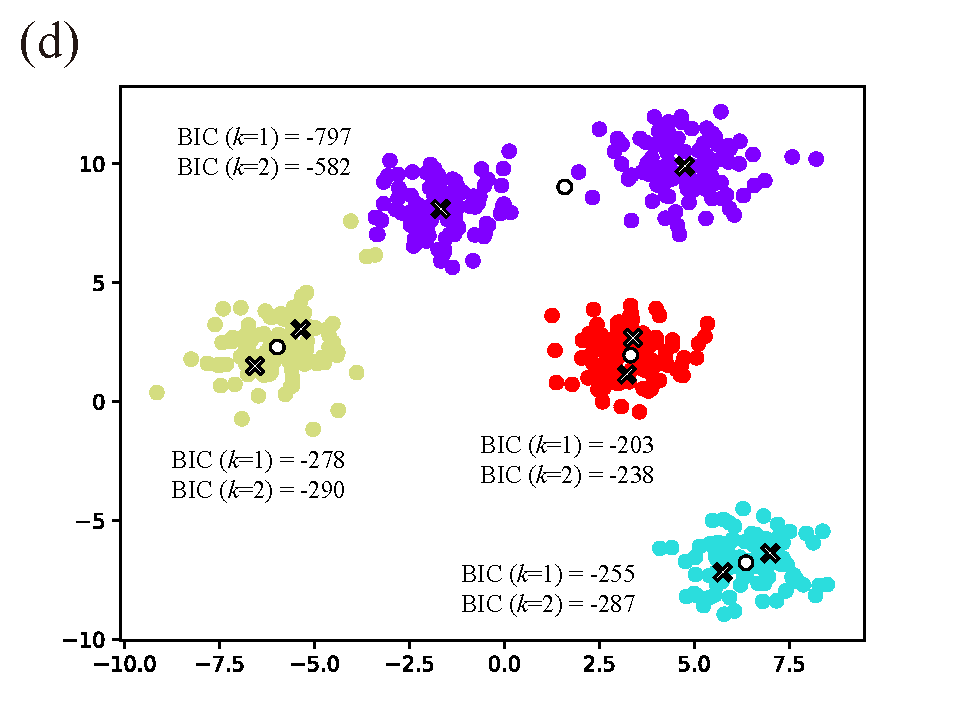
\includegraphics[width=1\linewidth]{img/xmeans/d.pdf}
    \end{center}
  \end{minipage}\\
  \begin{center}
    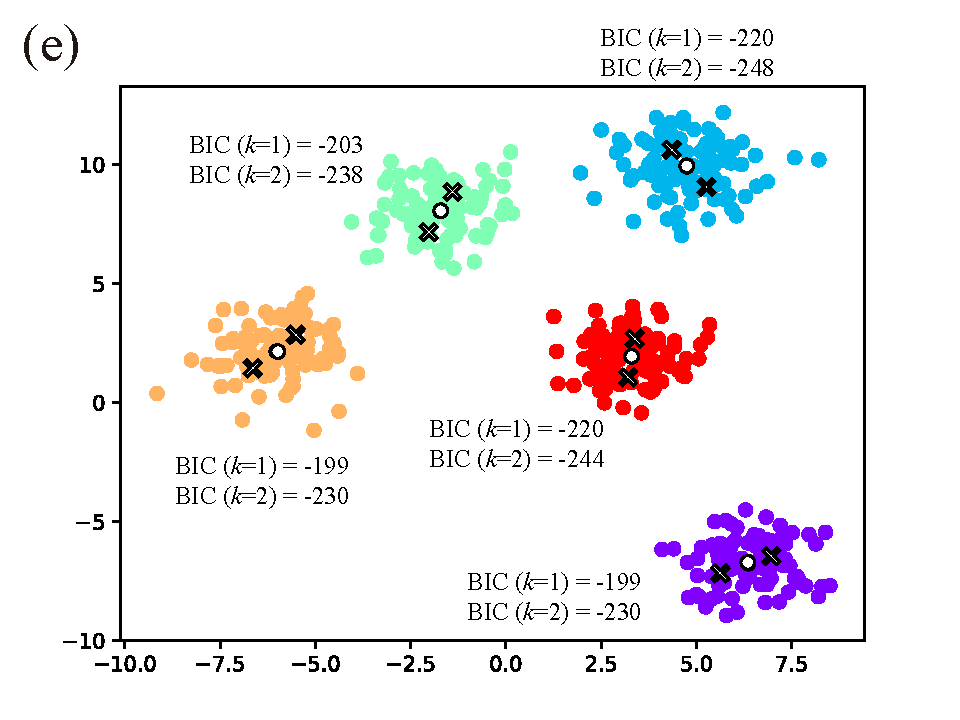
\includegraphics[width=0.5\linewidth]{img/xmeans/e.pdf}
  \end{center}
  \caption{X-meansの動作}
  \label{fig:x-means}
\end{figure}

X-meansで用いるBICは次のように求められる.
$d$次元のデータ${\bm D}=({\bm x_0}, {\bm x_1}, \cdots, {\bm x_d})$を
$K$個のクラスタに分割することを考える.
モデル$M_j$の評価に用いるBICは\eqref{eq:bic}で与えられる.
$p_j$はモデル$M_j$のパラメータ数であり,$R$は$M_j$のデータ数,
$\hat{l}_j(D)$は$p$変量Gauss分布の対数尤度関数である.

等方Gauss分布を考えると分散$\sigma^2$は\eqref{eq:variance}により表される.
\begin{align}
  \label{eq:variance}
  \hat{\sigma}^2 = \frac{1}{R-K}\sum_i\left({\bm x}_i-{\bm \mu}_{(i)}\right)^2
\end{align}
すると,確率は次で表される.
\begin{align}
  \label{eq:gaussian-distribution}
  \hat{P}(x_i) = \frac{R_{(i)}}{R}\frac{1}{\sqrt{2\pi}\hat{\sigma}^d}
    \exp\left(-\frac{1}{2\hat{\sigma}^2}||{\bm x}_i-{\bm \mu}_{(i)}||^2\right)
\end{align}
ここで${\bm \mu}_{i}$は$d$次元の平均ベクトルである.
したがって対数尤度関数は
\begin{align}
  \label{eq:log-likelihood}
  l(D) &= \log \prod_i \hat{P}(x_i) \\\nonumber
  &= \sum_i \left( \log\frac{1}{\sqrt{2\pi}\sigma^d}-\frac{1}{2\sigma^2}||{\bm x}_i-{\bm \mu}_{(i)}||^2 + \log\frac{R_{(i)}}{R} \right)
\end{align}
となる.
ここでクラスタ$n (1 \leq n \leq K)$のデータ$D_n$に着目する.
クラスタ$n$のデータ数を$R_n$と表記すると,\eqref{eq:log-likelihood}は以下で表される.
\begin{align}
  \begin{split}
    \hat{l}(D_n) &= -\frac{R_n}{2}\log(2\pi) - \frac{R_n \cdot d}{2}\log(\hat{\sigma}^2) -
    \frac{R_n - K}{2}\\ &
    + R_n\log R_n - R_n \log R
  \end{split}
\end{align}

一般的には,分割停止規準としてBICを用いるが,本実験においては,BIC以外の情報量規準を用いた
クラスタリングも行い,クラスタ数推定の精度を検証する.

\subsection{情報量規準}
情報量規準とは,最尤推定によって当てはめられたモデルが複数個あるときに,その中の一つを選択する規準である.

モデルの良し悪しは,最尤モデルの平均対数尤度のデータ$\vector{x}$に関する期待値
(期待平均対数尤度)によって考えることができる.
期待平均対数尤度の値が大きいほど,そのモデルは良いといえる.
モデルの最大対数尤度を期待平均対数尤度の1つの推定量と捉えることができるが,
詳しく調べると,最大対数尤度そのものは期待平均対数尤度の不偏推定量にならないことがわかる.
一般に最大対数尤度は,期待平均対数尤度の本当の値に比べて大きく出やすいという偏りを持つ.
この傾向はモデルの自由パラメータ数が大きいほど著しい.
これは最大対数尤度の比較に寄ってモデルを選択すると,自由パラメータ数の大きいモデルほど選ばれやすいことを示している.

最大対数尤度の期待平均対数尤度に対する偏りの程度とモデルの自由パラメータ間の関係を調べると,
\begin{align*}
  (モデルの最大尤度対数) - (モデルの自由パラメータ数)
\end{align*}
が近似的に期待平均対数尤度の不偏推定量となることが導かれる.
これがAICと呼ばれる情報量規準である.
AICを最大とするモデルが最適なモデルと考えられる.
AICは最大対数尤度が同程度のモデルがあるときには,その中で実際に推定しなければならないパラメータの数が
最も少ないものを選ぶべきであることを示している.

多くの情報量規準は,AICの形式を踏襲し,
\begin{align*}
  (モデルの最大尤度対数) - (モデルの自由パラメータ数などの罰則項)
\end{align*}
という形をしている.

以下に,いくつか情報量規準の例を示す.
なお,モデル$M_j$の$p_j$変量等方Gauss分布の対数尤度関数を$\hat{l}_j$と表し,
モデルのデータ数を$R$と表す.
\begin{description}
  \item[AIC (Akaike Information Criterion; 赤池情報量規準)]~\\
    1973年に赤池$^{2)}$によって提案された情報量規準である.
    \begin{align}
      \label{eq:aic}
      \mathrm{AIC}(M_j) = \hat{l}_j(D) - p_j
    \end{align}
  \item[cAIC (Conditional Akaike Information Criterion; 条件付き赤池情報量規準)]~\\
    AICは導出に漸近理論を使っているため,標本サイズが無限に大きいことを想定している.
    したがって,標本サイズが小さい場合はその過程が成り立たず,AICによるモデル決定は
    パラメータ数を過大に見積もってしまう.

    そこで,N. Sugiura$^{3)}$ は漸近理論を使わない不偏推定量であるcAICを導出した.
    \begin{align}
      \label{eq:caic}
      \mathrm{cAIC}(M_j) = \hat{l}_j(D) - \frac{p_j \cdot R}{R-p_j-1}
    \end{align}
  \item[BIC (Beyesian Information Criterion; ベイズ情報量規準)]~\\
    BICは1978年にSchwartz$^{4)}$によって提案された.
    AICとは異なり,罰則項に事後確率を利用する.
    \begin{align}
      \label{eq:bic}
      \mathrm{BIC}(M_j) = \hat{l}_j(D) - \frac{p_j}{2}\ln R
    \end{align}
  % TIC: https://repository.kulib.kyoto-u.ac.jp/dspace/bitstream/2433/155553/1/kronso_183_2_67.pdf
  % TIC, GIC: http://www.ism.ac.jp/editsec/toukei/pdf/47-2-375.pdf
  % \item[TIC (Takeuchi Information Criterion; 竹内情報量規準)]
  %   \begin{align}
  %     \label{eq:tic}
  %     \mathrm{TIC}(M_j) = \hat{l}_j(D) - \mathrm{Tr}(\hat{I}\hat{J}^{-1})
  %   \end{align}
  %   ここで,$\hat{I}$と$\hat{J}$はそれぞれ,
  %   \begin{align*}
  %     I_0 = E_g
  %   \end{align*}
\end{description}

